\chapter{I giochi con avversario}

I giochi che potremo esplorare hanno regole semplici e sono formalizzabili, in particolare avranno un ambiente accessibile e deterministico e vi saranno due giocatori con turni alterni, a \textbf{\textit{somma zero}}.\
Si tratta di giochi \textbf{a informazione perfetta}.

Siamo nel contesto di un ambiente multi-agente \textbf{\textit{competitivo}}:\ la presenza dell'avversario rende l'ambiente \textbf{\textit{strategico}} $\Rightarrow$ più difficile rispetto ai problemi di ricerca visto finora.\

Complessità e vincoli di tempo reale:\ la mossa migliore nel tempo disponibile.

\begin{center}
	\textit{I giochi sono un po' più simili ai problemi reali}.
\end{center}

\subsubsection{Ciclo pianifica-agisci-percepisci}

Caso di due agenti che agiscono ``a turno'':\ si può ancora pianificare considerando le possibili risposte dell'avversario e le possibili risposte a queste risposte\dots\

\noindent Una volta decisa la mossa migliore da fare:
\begin{itemize}
	\item si esegue la mossa,
	\item si vede cosa fa l'avversario,
	\item si ri-pianifica la prossima mossa.
\end{itemize}

\begin{figure}[H]
	\centering
	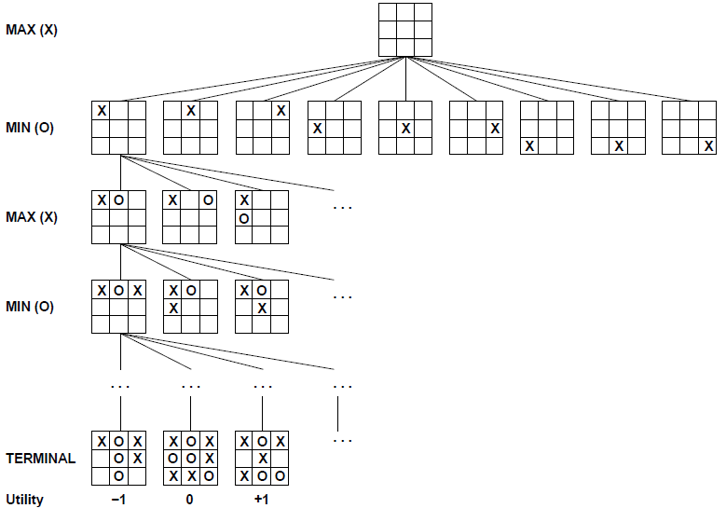
\includegraphics[width=0.8\textwidth]{immagini/TicTacToe.png}
	\caption*{Albero di gioco parziale}
\end{figure}

\section{Giochi come problemi di ricerca}

\begin{itemize}
	\item \textit{Stati}:\ configurazioni del gioco.
	\item \textit{Player}(\textit{s}):\ a chi tocca muovere nello stato \textit{s}.
	\item \textit{Stato iniziale}:\ configurazione iniziale del gioco.
	\item \textit{Actions}(\textit{s}):\ le mosse legali in \textit{s}.
	\item \textit{Result}(\textit{s,a}):\ lo stato risultante da una mossa, è il modello di transizione.
	\item \textit{Terminal-Test}(\textit{s}):\ determina la fine del gioco.
	\item \textit{Utility}(\textit{s, p}):\ funzione di \textit{utilità} (o \textit{pay-off}), valore numerico che valuta gli stati terminali del gioco per \textit{p}, per esempio $1|-1|0$, conteggio punti,\ \dots\ l'importante è che la somma sia costante.
\end{itemize}

\subsection{Algoritmo Min-Max}

\begin{figure}[H]
	\centering
	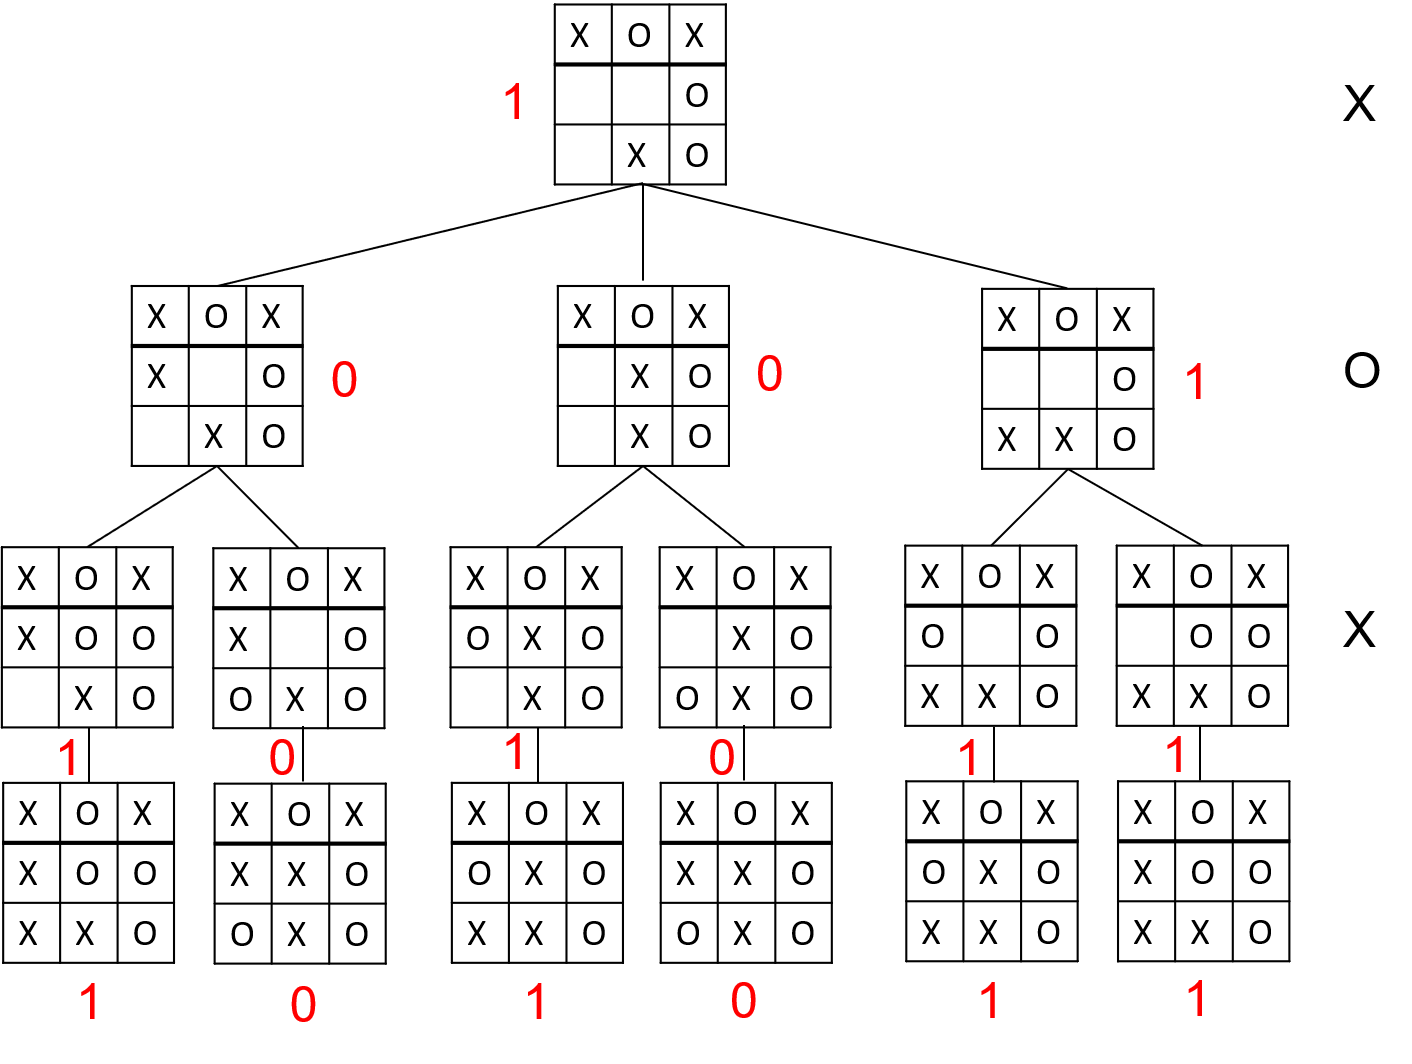
\includegraphics[width=0.8\textwidth]{immagini/TicTacToe_fine.png}
\end{figure}

\subsubsection{Esempio di una mossa (e contromossa)}

\begin{figure}[H]
	\centering
	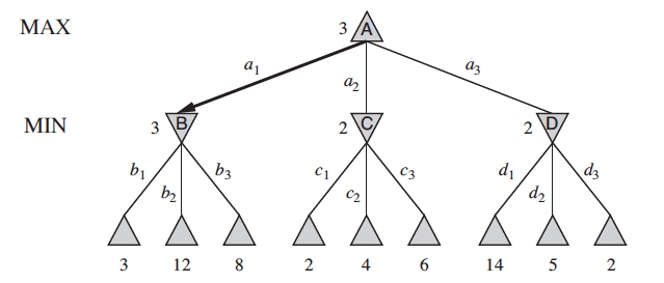
\includegraphics[width=0.5\textwidth]{immagini/MinMax.png}
	\caption*{Albero di gioco profondo ''una mossa'', due livelli o \textbf{\textit{ply}}}
\end{figure}

\noindent Calcolo del valore minimax dei nodi:\ il triangolo con la punta in su rappresenta un nodo MAX, mentre quello con la punta in giù un nodo MIN.\
Le foglie sono situazioni terminali di gioco.

\subsubsection{Valore Minimax}

Minimax(s) =
\begin{table}[H]
	\centering
	\begin{tabular}{l l}
		$Utility(s, \mathit{MAX})$                                                & $\mathrm{if}\ \mathit{Terminal\textrm{-}Test}(s)$          \\
		$\mathrm{\mathbf{max}}_{a \in Actions(s)} \mathrm{Minimax}(Result(s, a))$ & $\mathrm{if}\ \mathit{Player}(s) = \mathrm{\mathbf{MAX}}$  \\
		$\mathrm{\mathbf{min}}_{a \in Actions(s)} \mathrm{Minimax}(Result(s, a))$ & $ \mathrm{if}\ \mathit{Player}(s) = \mathrm{\mathbf{MIN}}$ \\
	\end{tabular}
\end{table}

\noindent Ma come conviene esplorare l'albero di gioco?

\begin{figure}[H]
	\centering
	\caption*{Algoritmo MIN-MAX ricorsivo}
	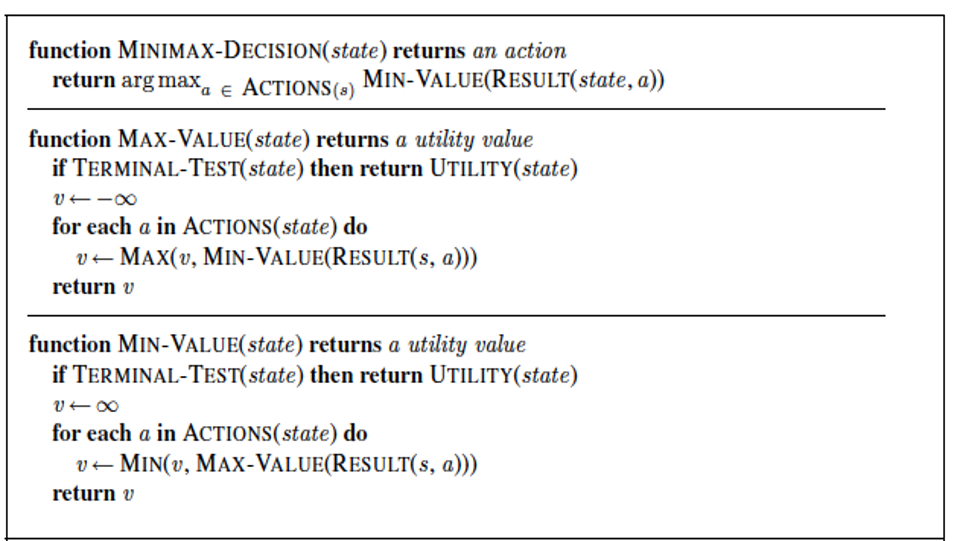
\includegraphics[width=\textwidth]{immagini/MinMax_rec.png}
\end{figure}

\subsubsection{Costo}

Tempo:\ come DF, $O(b^m)$; spazio:\ $O(m)$.

Scacchi:\ $35^{100}$ (35 mosse in media; 50 mosse per player); grafo degli scacchi $10^{40}$ nodi $\rightarrow\ 10^{22}$ secoli!

Improponibile un'esplorazione sistematica del grafo degli stati, se non per giochi veramente semplici (come il filetto).\
È necessario fare uso di \textbf{euristiche} per stimare la bontà di uno stato del gioco.

\subsubsection{Min-Max euristico (con orizzonte)}

In casi più complessi occorre una \textbf{funzione di valutazione euristica} dello stato, $Eval(s)$.\
Strategia:\ guardare avanti \textit{d} livelli
\begin{itemize}
	\item si espande l'albero di ricerca un certo numero di livelli \textit{d} (compatibile col tempo e lo spazio disponibili),
	\item si valutano gli stati ottenuti e si propaga indietro il risultato con la regola del MAX e MIN.
\end{itemize}
Algoritmo MIN-MAX come prima ma\dots

\begin{flushleft}
	\textbf{if} $Terminal-Test(s)$ \textbf{then return} $Utility(s)$ diventa

	\textbf{if} \textit{Cutoff-Test}(\textit{s,d}) \textbf{then return} $Eval(s)$
\end{flushleft}
\textbf{\textit{Cutoff-Test}} riconosce stati terminali.

\subsubsection{Valore H-Minimax}
Se \textit{d} è il limite alla profondità consentita …

\noindent H-Minimax(s, d) =

\begin{table}[H]
	\centering
	\begin{tabular}{l l}
		$Eval(s)$                                                                                  & $\mathrm{if}\ \mathit{Cutoff\textrm{-}Test}(s,d)$         \\
		$\mathrm{max}_{a \in Actions(s)} \mathrm{H\textrm{-}Minimax}(\mathit{Result}(s, a), d +1)$ & $\mathrm{if}\ \mathit{Player}(s) = \mathrm{\mathbf{MAX}}$ \\
		$\mathrm{min}_{a \in Actions(s)} \mathrm{H\textrm{-}Minimax}(\mathit{Result}(s, a), d +1)$ & $\mathrm{if}\ \mathit{Player}(s) = \mathrm{\mathbf{MIN}}$ \\
	\end{tabular}
\end{table}

\subsubsection{Il filetto}

$Eval(s) = X(s) - O(s)$
\begin{itemize}
	\item $X(s)$:\ righe aperte per X
	\item $O(s)$:\ righe aperte per O
\end{itemize}
Una configurazione vincente per X viene stimata $+\infty$, una vincente per O $-\infty$.

\subsubsection{La funzione di valutazione}

La funzione di valutazione \textit{Eval} è una \textbf{stima della utilità attesa} a partire da una certa posizione.\
La qualità della \textit{funzione} è determinante:
\begin{itemize}
	\item deve essere consistente con l'utilità se applicata a stati terminali del gioco (indurre lo stesso ordinamento);
	\item deve essere efficiente da calcolare;
	\item deve riflettere le probabilità effettive di vittoria (A valutato meglio di B se da A ci sono più probabilità di vittoria che da B);
	\item valore ``atteso'' che combina probabilità con utilità dello stato terminale, può essere appreso con l'esperienza.
\end{itemize}

\noindent Per gli scacchi si potrebbe pensare di valutare caratteristiche diverse dello stato:
\begin{itemize}
	\item Valore del materiale (pedone 1, cavallo o alfiere 3, torre 5, regina 9,\ \dots)
	\item Buona disposizione dei pedoni, protezione del re
\end{itemize}

\noindent Una funzione lineare pesata potrebbe essere
\[
	Eval(s) = w_1 f_1(s) + w_2 f_2(s) + \dots + w_n f_n(s)
\]
\begin{itemize}
	\item []$f_i$:\ caratteristica (es.\ numero dei pezzi)
	\item[] $w_i$:\ peso relativo (es.\ valore dei pezzi)
\end{itemize}

\noindent È possibile avere anche combinazioni non lineari di caratteristiche:\ alfiere vale più nei finali di partita, 2 alfieri valgono più del doppio di 1.

\subsubsection{Problemi con MIN-MAX:\ Stati non quiescienti}
\textit{Stati non quiescienti}:\ l'esplorazione fino ad un livello può mostrare una situazione molto vantaggiosa, poi alla mossa successiva la regina nera viene catturata.\

\textit{Soluzione}:\ applicare la valutazione a stati \textit{quiescenti}, stati in cui la funzione di valutazione non è soggetta a mutamenti repentini (ricerca di quiescenza).\

\subsubsection{Problemi con MIN-MAX:\ Effetto orizzonte}
\textit{Effetto orizzonte}:\ può succedere che vengano privilegiate mosse diversive che hanno il solo effetto di spingere il problema oltre l'orizzonte.\

\begin{figure}[H]
	\centering
	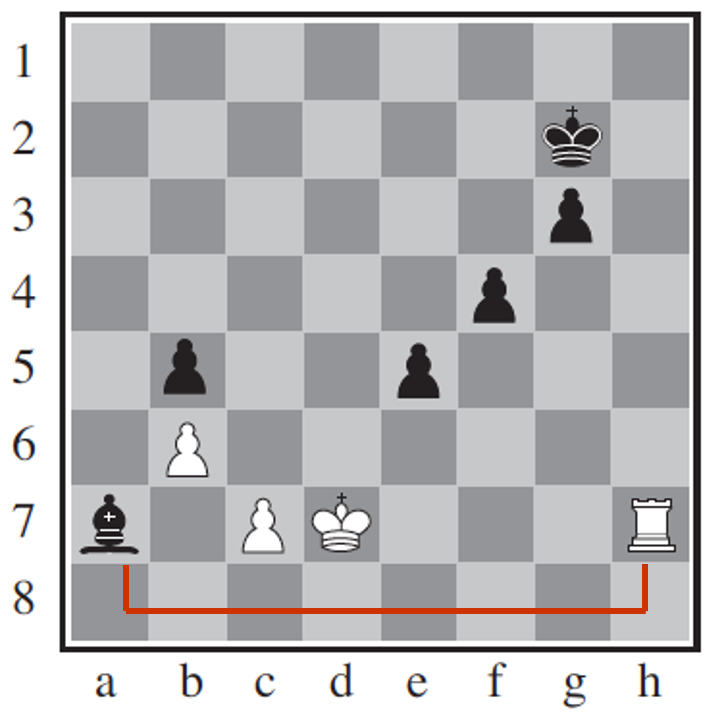
\includegraphics[width=0.4\textwidth]{immagini/EffettoOrizzonte.png}
\end{figure}

\noindent L'alfiere in A7, catturabile in 3 mosse dalla torre, è spacciato.\
Mettere il re bianco sotto scacco con il pedone in E5 e poi con quello in F4\dots\ evita il problema temporaneamente, ma è un sacrificio inutile di pedoni.\

\subsubsection{Ottimizzazione}
Ma dobbiamo necessarimente esplorare ogni cammino?\
No, esiste un modo di dimezzare la ricerca pur mantenendo la decisione minimax corretta:\ Potatura alfa-beta (McCarthy 1956, per scacchi).

\subsection{Potatura alfa-beta}

Tecnica di \textit{potatura} per ridurre l'esplorazione dello spazio di ricerca in algoritmi MIN-MAX.

\begin{figure}[H]
	\centering
	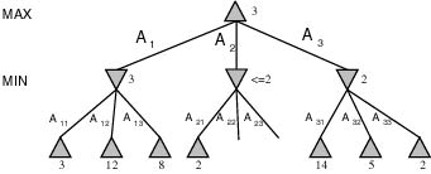
\includegraphics[width=0.6\textwidth]{immagini/alfaBeta_idea.jpg}
\end{figure}

\begin{table}[H]
	\centering
	\begin{tabular}{l l}
		MINMAX(\textit{radice}) & $ = \max(\min (3,12,8),\ \min(2,x,y),\ \min(14,5,2))$ \\
		                        & $= \max (3,\ \min(2, x, y),\ 2) $                     \\
		                        & $ = \max(3, z, 2) = 3$ \qquad	con $z \leq 2 $
	\end{tabular}
\end{table}
\noindent \textbf{Nota}:\ il risultato è lo stesso ma la ricerca è più efficiente; sperimentalmente si è visto che si può raddoppiare il numero di nodi esplorati a parità di risorse spazio-temporali.\

\noindent Più in generale, consideriamo un valore \textit{v} trovato a una certa profondità.\
Se c'è una scelta migliore, $\alpha$, a profondità minore, quel \textit{v} non sarà mai raggiunto:\ MAX passerà da $\alpha$ piuttosto che finire a \textit{v}.

\subsubsection{Implementazione}
Si va avanti in profondità fino al livello desiderato e propagando indietro i valori si decide se si può abbandonare l'esplorazione nel sotto-albero.\

MaxValue e MinValue vengono invocate con due valori di riferimento:\ $\alpha$ (inizialmente $-\infty$) e $\beta$ (inizialmente $+\infty$) che rappresentano rispettivamente la migliore alternativa per MAX e per MIN fino a quel momento.\
I tagli avvengono quando nel propagare indietro:
\begin{itemize}
	\item $v \geq \beta$ \qquad per i nodi MAX (taglio $\beta$)
	\item $v \leq \alpha$ \qquad per i nodi MIN (taglio $\alpha$)
\end{itemize}

\begin{figure}[H]
	\centering
	\caption*{L'algoritmo Alfa-Beta}
	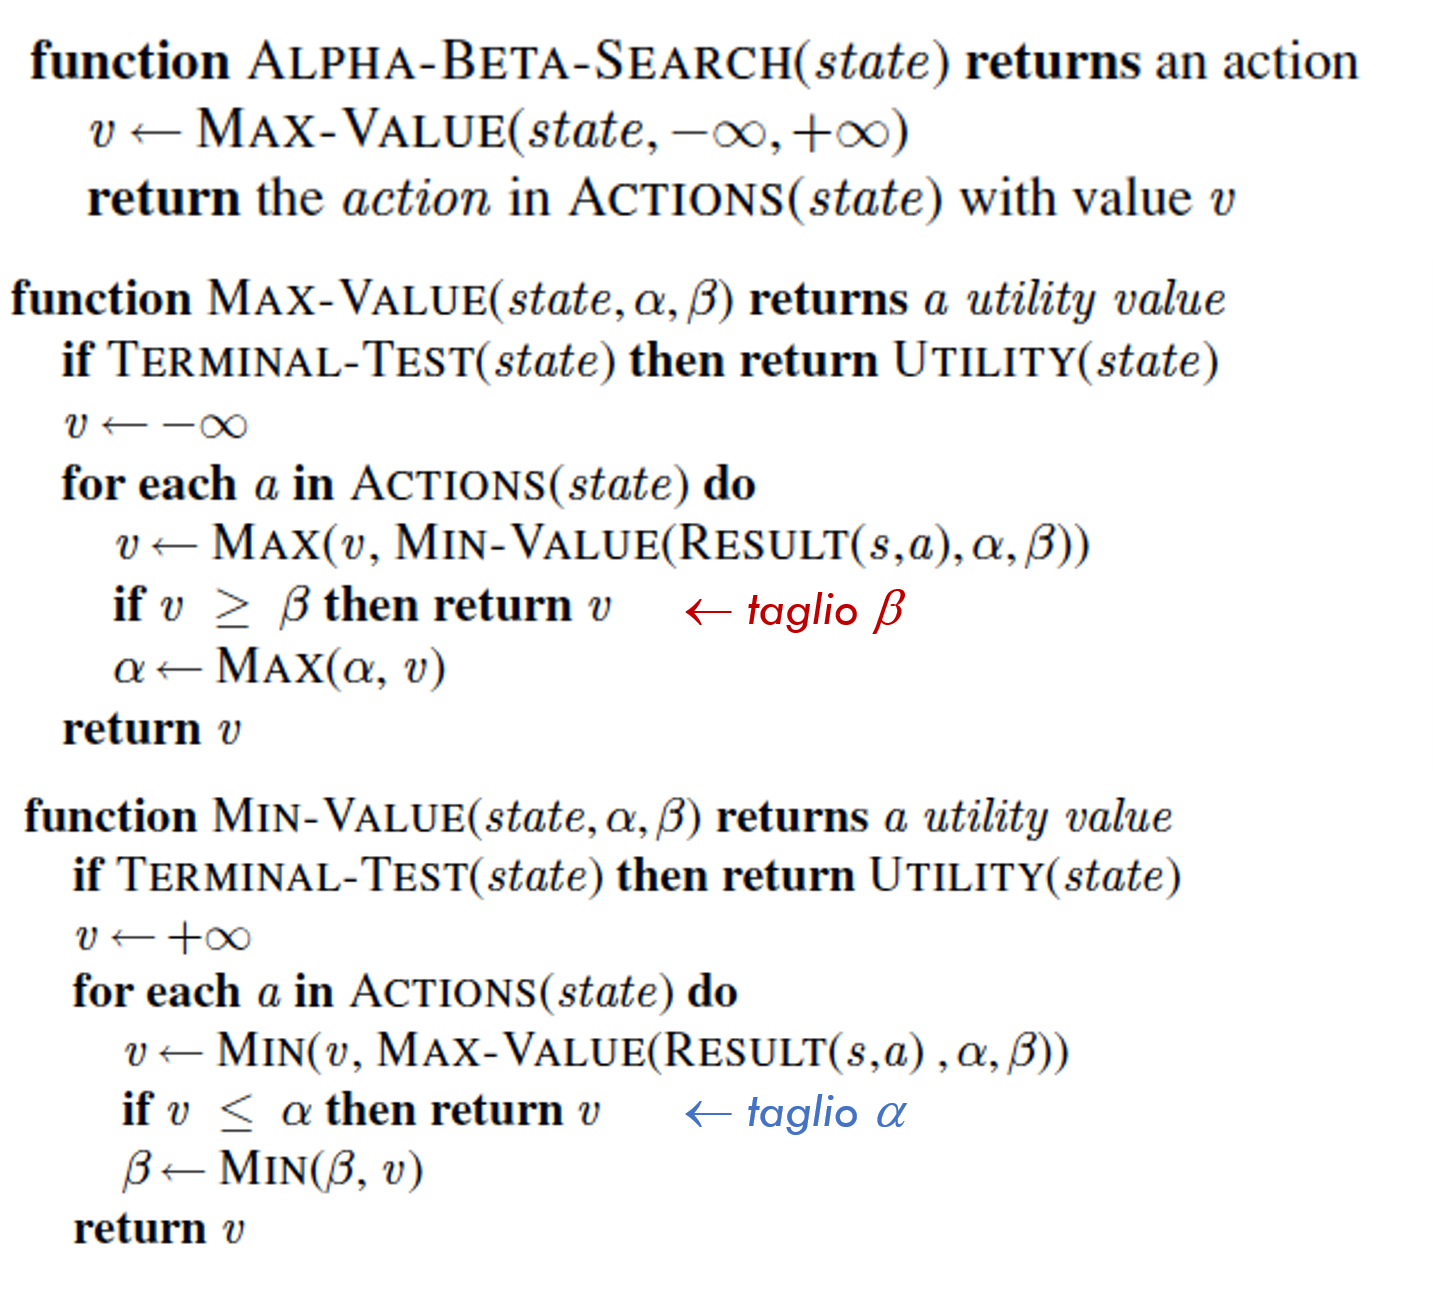
\includegraphics[width=0.7\textwidth]{immagini/AlfaBeta_alg.png}
\end{figure}

\begin{figure}[H]
	\centering
	\caption*{Alfa-beta in azione}
	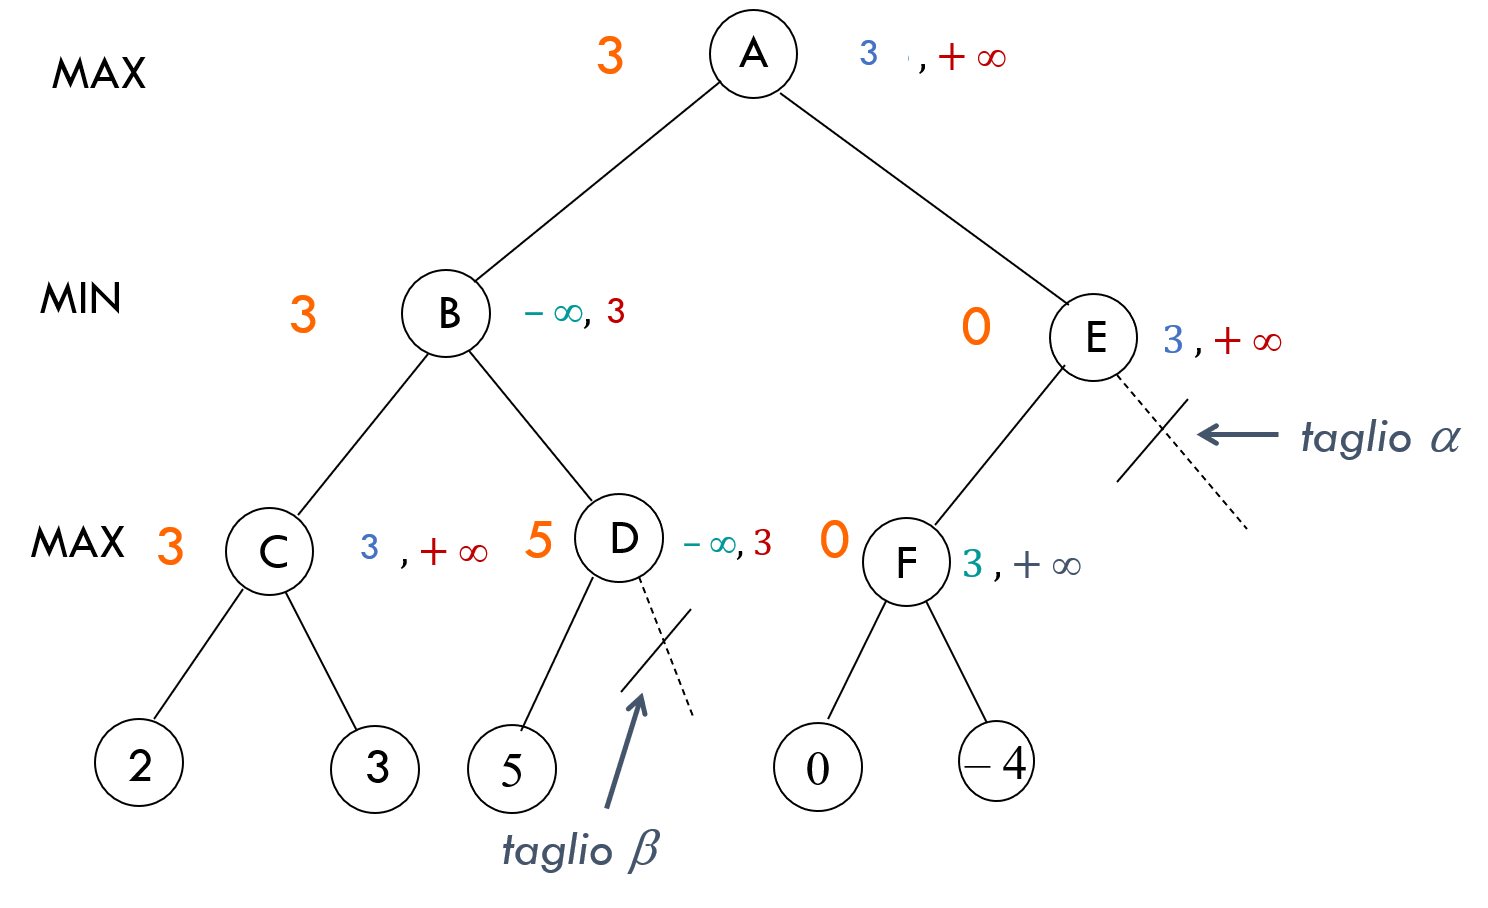
\includegraphics[width=0.7\textwidth]{immagini/alfaBeta_azione.jpg.png}
\end{figure}

\noindent \textbf{Nota bene}:\ i nodi sotto vengono visitati (esamina alcuni discendenti per raccogliere le info) come che D vale 5 e F 0 e -4\dots\
Il taglio è cioè sotto la linea indicata!\
Ma è qua il senso importante:\ si tagliano sottolaberi come quello radicato in G a destra perché $\alpha$ e $\beta$ risalgono.

\subsubsection{Ordinamento delle mosse}

La potatura ottimale si ottiene quando ad ogni livello sono generate prima le mosse migliori per chi gioca:\ per nodi MAX sono generate prima le mosse con valore più alto, mentre per i nodi MIN sono generate prima le mosse con valore più basso (migliori per MIN).

\textbf{Complessità}:\ $O(b^{m/2})$ anziché $O(b^m)$.\

\noindent Alfa-Beta può arrivare a profondità doppia rispetto a Min-Max!\
Ma come avvicinarsi all'ordinamento ottimale?\
Ordinamento dinamico:

\begin{itemize}
	\item Usando approfondimento iterativo si possono scoprire ad una iterazione informazioni utili per l'ordinamento delle mosse, da usare in una successiva iterazione (mosse killer).
	\item Tabella delle trasposizioni:\ per ogni stato incontrato si memorizza la sua valutazione.\
	      Situazione tipica:\ [a\textsubscript{1}, b\textsubscript{1}, a\textsubscript{2}, b\textsubscript{2}] e [a\textsubscript{1}, b\textsubscript{2}, a\textsubscript{2}, b\textsubscript{1}] portano nello stesso stato.
\end{itemize}

\subsubsection{Altri miglioramenti}

Potatura in avanti:\ esplorare solo alcune mosse ritenute promettenti e tagliare le altre.
\begin{itemize}
	\item Beam search;
	\item Tagli probabilistici (basati su esperienza).\ Miglioramenti notevoli in Logistello.
\end{itemize}
Database di mosse di apertura e chiusura:
\begin{itemize}
	\item Nelle prime fasi ci sono poche mosse sensate e ben studiate, inutile esplorarle tutte.\
	\item Per le fasi finali il computer può esplorare off-line in maniera esaustiva e ricordarsi le migliori chiusure (già esplorate tutte le chiusure con 5 e 6 pezzi\dots).
\end{itemize}

\section{Problemi di soddisfacimento di vincoli}
Sono problemi con una struttura particolare, che si prestano ad algoritmi di ricerca specializzati.\
È un esempio di rappresentazione \textbf{fattorizzata}, in cui si comincia a dire qualcosa sulla struttura dello stato.\
Esistono euristiche generali che si applicano e che consentono la risoluzione di problemi di dimensioni significative per questa classe.\
La classe di problemi formulabili in questo modo è piuttosto ampia:\ layout di circuiti, scheduling,\ \dots

\subsubsection{Formulazione di problemi CSP}

\textit{Problema}:\ descritto da tre componenti
\begin{enumerate}
	\item X un insieme di variabili.
	\item D un insieme di domini, dove D\textsubscript{i} è l'insieme dei valori possibili per X\textsubscript{i}.
	\item C un insieme di vincoli (relazioni tra le variabili).
\end{enumerate}
\begin{flushleft}
	\textit{Stato}:\ un assegnamento [\textbf{parziale}$|$\textbf{completo}] di valori a variabili
	\[
		\{X_i = v_i ,\ X_j = v_j,\ \dots\}
	\]

	\textit{Stato iniziale}:\ \{ \}

	\textit{Azioni}:\ assegnamento di un valore a una variabile (tra quelli leciti)

	\textit{Soluzione} (goal test):\
	un assegnamento \textbf{completo} (le variabili hanno tutte un valore) e \textbf{consistente} (i vincoli sono tutti soddisfatti).
\end{flushleft}

\subsection{Strategie per problemi CSP}

Finora potevamo solo ricercare la soluzione nel grafo degli stati (guidati da una metrica definita sullo stato).\
Adesso possiamo
\begin{itemize}
	\item usare delle euristiche specifiche per questa classe di problemi;
	\item fare delle inferenze che ci portano a restringere i domini e quindi a limitare la ricerca:\ \textbf{\textit{propagazione di vincoli}};
	\item fare backtracking \textbf{\textit{intelligente}}.
\end{itemize}
Tipicamente un misto di queste strategie.

\subsection{Ricerca in problemi CSP}
Ad ogni passo si assegna una variabile.\
La massima profondità della ricerca è fissata dal numero di variabili \textit{n}.\
Versione ``ingenua'':
\begin{itemize}
	\item l'ampiezza dello spazio di ricerca è $|D_1|\times|D_2|\times\ \dots\ \times|D_n|$ dove $|D_i|$ è la cardinalità del dominio di X\textsubscript{i},
	\item il fattore di diramazione è pari a $nd$ al primo passo; $(n-1) d$ al secondo\dots\ le foglie sarebbero $n! \cdot d^n$.
\end{itemize}
Riduzione drastica dello spazio di ricerca dovuta al fatto che il \textit{goal-test} è commutativo, non è importante l'ordine con cui scelgo le variabili quindi ad ogni livello posso scegliere una e una sola variabile per un fattore di diramazione pari a \textit{d}.\
In realtà il fattore di diramazione è pari alla dimensione dei domini \textit{d} ($d^n$ foglie).

\subsubsection{Strategie di ricerca}
Ricerca con \textit{backtracking} (BT) a profondità limitata.\
\textbf{\textit{Controllo anticipato}} della violazione dei vincoli:\ è inutile andare avanti fino alla fine e poi controllare; si può fare \textit{backtracking} non appena si scopre che un vincolo è stato violato.\

La ricerca è limitata naturalmente in profondità dal numero di variabili quindi il metodo è completo.\

\begin{figure}[H]
	\centering
	\caption*{Backtracking ricorsivo per CSP}
	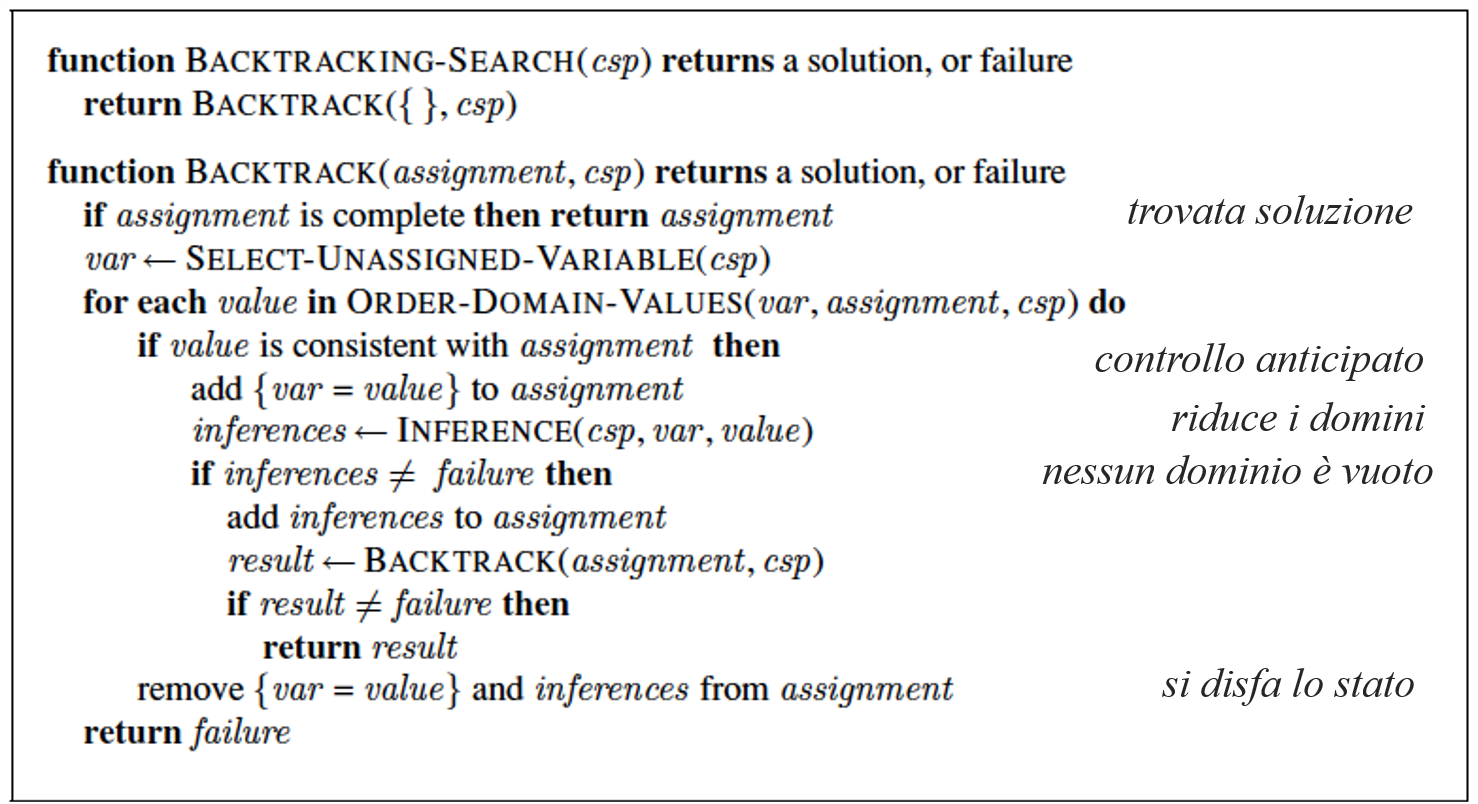
\includegraphics[width=0.9\textwidth]{immagini/Backtracking_rec.png}
\end{figure}

\noindent\textbf{SelectUnassignedVariable}:\ Quale variabile scegliere?

\noindent\textbf{OrderDomainValues}:\ Quali valori scegliere?

\noindent\textbf{Inference}:\ Qual è l'influenza di un assegnamento sulle altre variabili?\ Come restringe i domini?\ \textit{Propagazione di vincoli}, \textit{riduzione problema}.

\noindent\textbf{BackTrack}:\ Come evitare di ripetere i fallimenti?\ \textit{Backtracking intelligente}.

\subsubsection{Scelta delle variabili}

\begin{enumerate}
	\item MRV (\textit{Minimum Remaining Values}):\ scegliere la variabile che ha meno valori legali [residui], la variabile \textbf{\textit{più vincolata}}.\ Si scoprono prima i fallimenti (\textit{fail first}).
	\item Euristica \textit{del grado}:\ scegliere la variabile coinvolta in più vincoli con le altre variabili (\textit{la variabile \textbf{più vincolante}} o di \textit{grado maggiore}).\ Da usare a parità di MRV.
\end{enumerate}

\subsubsection{Scelta dei valori}

Una volta scelta la variabile come scegliere il valore da assegnare?\

Valore \textbf{\textit{meno vincolante}}:\ quello che esclude meno valori per le altre variabili direttamente collegate con la variabile scelta, meglio valutare prima un assegnamento che ha più probabilità di successo.\
Se volessimo tutte le soluzioni l'ordine non sarebbe importante.

\subsubsection{Propagazione di vincoli}

\begin{enumerate}
	\item Verifica in avanti (\textit{Forward Checking} o \textit{FC}):\ assegnato un valore ad una variabile si possono eliminare i valori incompatibili per le altre variabili \textbf{\textit{direttamente collegate}} da vincoli (non si itera).
	\item Consistenza di nodo e d'arco:\ si restringono il valori dei domini delle variabili tenendo conto dei vincoli unari e binari su tutto il grafo (si itera finché tutti i nodi ed archi sono consistenti).
\end{enumerate}

